\chapter{ZX-Calculus: First Contact}

% \begin{lstlisting}[language = Python]
% import pyzx
% \end{lstlisting}

To study quantum computing, we have a few special-purpose notations:
\begin{itemize}[leftmargin = *]
    \item \textbf{Quantum Circuits:} This notation studies quantum computing on an implementation level. It explores the components required to build quantum circuits and their \textit{tuning} for optimal performance. This involves both designing and hardware implementation of quantum circuits.   
    \item \textbf{Measurement Calculus:} This notation entails a mathematical study of quantum circuits. Making use of mathematical tools, it studies the \textit{manipulation} of quantum data at different stages of quantum circuits. 
\end{itemize}

ZX-calculus falls in the second category of notations. It makes use of the complementarity of Z-basis and X-basis, and defines the quantum circuits in a graphical language so that they are more mathematically elaborate. The advantage is the understanding of quantum algorithms beyond gate-level implementation -- among many.

This chapter is dedicated as an introduction to the notation of ZX-Calculus and its elements. It will make use of PyZX, a Python package for ZX-Calculus, to provide an early acquaintance to this tool. PyZX itself will be explored in more detail in the next chapter.  

\section{PyZX: Python Library for ZX-Calculus}
As we mentioned in chapter \ref{ch:python}, programming is a tool used by engineers, scientists, and pretty much everyone for assistance in computation. We also introduced you to libraries with the promise that we will be using them often. In fact, we will be actively working with coding throughout this book.

PyZX (pronounced as `pixie') is a python library for assisting with the visualisation of ZX-calculus diagrammatics and for computationally optimising the ZX-graphs.

For installing PyZX, run the following command using either the terminal or your Jupyter notebook:
\begin{python}
pip install pyzx
\end{python}

Once installed, you can use PyZX in your Python program by importing it. For that, use: 

\begin{python}
import pyzx
\end{python}

We will not dive into PyZX any deeper in this chapter and will come back to it in chapter \ref{ch:pyzx} when we are in a better position of understanding ZX-Calculus and appreciating PyZX. For now, this much detail will suffice for our working.  

\section{Building Blocks}
The ZX-Calculus language is composed of several building blocks which connect together to form the diagrams. As the ZX-Calculus is a graphical diagramamtic language, it chiefly consists of nodes and edges. We will explain them one by one in this section:

\subsection{Wires}
You may have known about electric wires from the circuits in your home and from your science books; they are used to connect the components of an electrical circuit together. Very much like that, we have wires in ZX-Calculus language to connect different components together. However, do not think them of a carrier of electrons like in a classical electrical circuit. Instead, these are like the \textit{edges} of a graph, connecting different nodes together.  
 
Diagrammatically, wires are simply black lines. Let's use the following code to see what wires look like in PyZX:

\begin{python}
# Instantiate an empty graph
g = pyzx.Graph()
# Add vertices using the following command:
i =  g.add_vertex(0, 0, 0)
o =  g.add_vertex(0, 0, 3)
g.add_edges([(i,o)])
# Then draw it
display(pyzx.draw(g))
\end{python}

Here's the output obtained by running the code:
\[
\begin{tikzpicture}[tikzfig]
    \begin{pgfonlayer}{nodelayer}
        \node [style=none] (0) at (0.00, 0.00) {};
        \node [style=none] (1) at (5.00, 0.00) {};
    \end{pgfonlayer}
    \begin{pgfonlayer}{edgelayer}
        \draw (0) to (1);
    \end{pgfonlayer}
\end{tikzpicture}
\]

This is the usual output obtained by using PyZX. However, the lines can be curved as well. One may as well draw the lines freehand as long as they follow the expected path.

\begin{minipage}{\linewidth}
    \begin{equation*}
        \tikzfig{Figures/wires}
    \end{equation*}
    \captionof{figure}{All the wires in this figure have the same meaning diagrammatically. Although they have different shapes, they all depict a simple circuit in which the input and output are directly connected.}
\end{minipage}

\subsection{Z($\alpha$) Vertices}
$Z_m^n$ are green-coloured vertices which have $m$ inputs and $n$ outputs. $m$ and $n$ can take non-zero integral values, even 0.

Let's make a $Z_0^0$ vertex using PyZX. For this, run the following code in Python.

\begin{python}
# Instantiate an empty graph
g = pyzx.Graph()
# Add vertices using the following command:
#   add_vertex(vertex_type, qubit_num, row_num, phase)
i = g.add_vertex(1, 0, 0)
# Then draw it
display(pyzx.draw(g))
\end{python}

This is the output of the code.
\[
\begin{tikzpicture}
\begin{pgfonlayer}{nodelayer}        
\node [style=Z dot] (0) at (0.00, 0.00) {};
\end{pgfonlayer}
\begin{pgfonlayer}{edgelayer}   
\end{pgfonlayer}
\end{tikzpicture}
\]

Z vertices also take a phase $\alpha$ as a parameter. The default value of the phase is 0. The significance of this phase will be explained in the next section.

Let's make a $Z_0^0(\nicefrac{\pi}{2})$ vertex using PyZX. As Python itself does not have have the value of pi stored, we will have to use the numpy library. For that, install numpy by running

\begin{python}
pip install numpy
\end{python}

and then import it using
\begin{python}
import numpy as np
\end{python}

Now, we can add the vertex by using the following code:
\begin{python}
#   add_vertex(vertex_type, qubit_num, row_num, phase)
g.add_vertex(1, 0, 0, np.pi/2)
\end{python}

\begin{equation*}
\begin{tikzpicture}[tikzfig]
\begin{pgfonlayer}{nodelayer}
\node [style=Z dot] (0) at (0.00, 0.00) {\param{\pi/2}};
\end{pgfonlayer}
\end{tikzpicture}
\end{equation*}

{
\begin{center}
\fcolorbox{black}{shadecolor}{%

    \parbox{\textwidth}
    {%
        \small
        {
            \textbf{Note:}\\
            When running the code on Python, you will not see the value as exactly $\nicefrac{\pi}{2}.$ Instead, it will appear as a fractional approximation. This is completely expected and should not put you off when you run the code.
        }
    }%
}
\end{center}
}

We will explain the Z vertex further in the coming sections, so bear with us as we first introduce you to other vertices in the ZX-language. 

% X(a)
\subsection{{X($\alpha$) Vertices}}
$X_m^n$ is a red-coloured vertex having $m$ inputs and $n$ outputs. Just like $Z_m^n$-vertices, $m$ and $n$ can take non-zero integral values, even 0.

To make a $X_0^0$ vertex using PyZX, run the following code in Python:

\begin{python}
# Instantiate an empty graph
g = pyzx.Graph()
# Add vertices using the following command:
#   add_vertex(vertex_type, qubit_num, row_num, phase)
i = g.add_vertex(2, 0, 0)
# Then draw it
display(pyzx.draw(g))
\end{python}

\[
\begin{tikzpicture}
    \begin{pgfonlayer}{nodelayer}        
        \node [style=X dot] (0) at (0.00, 0.00) {};
    \end{pgfonlayer}
\end{tikzpicture}
\]

Similarly, an $X_0^0(\alpha)$ vertex can be generated by using:
\begin{python}
g.add_vertex(2, 0, 0, np.pi)
\end{python}

\begin{equation*}
\begin{tikzpicture}[tikzfig]
\begin{pgfonlayer}{nodelayer}
\node [style=X dot] (0) at (0.00, 0.00) {\param{\pi}};
\end{pgfonlayer}
\end{tikzpicture}
\end{equation*}

\subsection{{H Vertices}}
$H$ vertices are yellow square-shaped vertices which have only one input and one output. They signify the Hadamard transform and can be written in matrix notation as
\begin{equation*}
    \dfrac{1}{\sqrt{2}}
    \begin{pmatrix}
        1 & 0\\
        0 & -1
    \end{pmatrix}
\end{equation*}

To make an $H$-vertex using Python, run the follwoing code:
\begin{python}
# Instantiate an empty graph
g = pyzx.Graph()
# Add vertices using the following command:
i = g.add_vertex(3, 0, 0)
# Then draw it
display(pyzx.draw(g))
\end{python}

\[
\begin{tikzpicture}[tikzfig]
\begin{pgfonlayer}{nodelayer}
    \node [style=none] (0) at (0.00, 0.00) {};
    \node [style=H] (1) at (0.00, 1.00) {};
    \node [style=none] (2) at (0.00, 2.00) {};
\end{pgfonlayer}
\begin{pgfonlayer}{edgelayer}
    \draw (0) to (1);
    \draw (2) to (1);
\end{pgfonlayer}
\end{tikzpicture}
\]

\subsection{$\sqrt{D}$ Vertices}
A $\sqrt{D}$ vertex is a black diamond-shaped vertex. It has no input or output.

\[
\begin{tikzpicture}[tikzfig]
\begin{pgfonlayer}{nodelayer}
    \node [style=D] (0) at (0.00, 0.00) {};
    \end{pgfonlayer}
\end{tikzpicture}
\]

{
\begin{center}
\fcolorbox{black}{shadecolor}{%

    \parbox{\textwidth}
    {%
        \small
        {
            \textbf{Note:}\\
           All these building blocks of ZX-Calculus -- the wires and the vertices -- are called \emph{generators} and are used to contruct ZX-diagrams, as we will see in the next section. 
        }
    }%
}
\end{center}
}

\section{Circuits Notation}
In ZX-calculus, the diagrams are enclosed in a box with a network of wires and vertices in it. This box is called the \emph{interface} through which the input and output pass through the circuit and through which we can connect other diagrams to the existing circuit. Thus, the simplest diagram would be the input and output connected together, as shown in fig. \ref{fig:diag1} i.e. the qubit goes through the circuit unprocessed. You can think of it in matrix notation as the identity matrix $$\begin{pmatrix}
    1 & 0\\
    0 &1
\end{pmatrix}.$$  
\begin{figure}[ht]
    \centering
    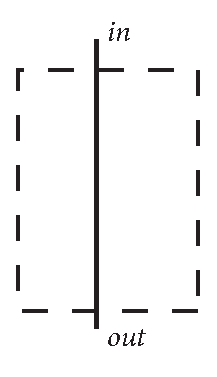
\includegraphics[scale = 0.55]{diag1}
    \caption{A simple ZX-diagram consisting of a single wire connecting input and output}
    \label{fig:diag1}
\end{figure}

A 2-qubit version would be having two wires passing through the circuit as shown in fig. \ref{fig:wires2}. This can be represented by an $I_4$ matrix $$\begin{pmatrix}
    1 & 0 & 0 & 0\\
    0 & 1 & 0 & 0\\
    0 & 0 & 1 & 0\\
    0 & 0 & 0 & 1
\end{pmatrix}.$$ 

\begin{figure}[ht]
    \centering
    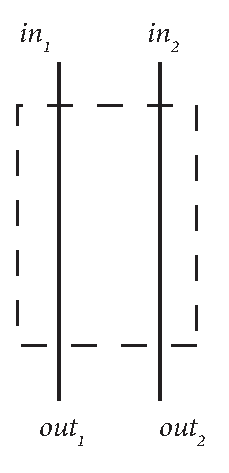
\includegraphics[scale = 0.45]{Figures/wires2-straight.eps}
    \caption{A ZX-circuit having two input/output connections.}
    \label{fig:wires2}
\end{figure}

Remember that we mentioned earlier that the shape of the wires do not matter. It is also worth noting that the overlapping paths of the wires do not matter either, hence the circuit in fig. \ref{fig:wires2-overlap} is the same as the one in fig. \ref{fig:wires2}.

\begin{figure}[ht]
    \centering
    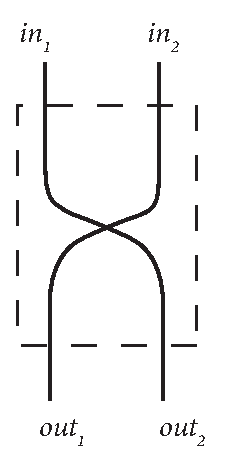
\includegraphics[scale=0.45]{wires2}
    \caption{In ZX-calculus notation, the wires can overlap without being ``shorted". Hence, this figure shows an $I_4$ circuit.}
    \label{fig:wires2-overlap}
\end{figure}

Notice the size of the matrices; the circuit with 1 wire from input to output has a matrix representation if size $2$-by$2$ while the one with two wires is 4-by-4. In fact, 

The 2-by-2 matrix represents the transformation of a 2-by-1 statevector to another 2-by-1 vector such that

\begin{align*}
    \begin{pmatrix}
        1 & 0\\
        0 & 1
    \end{pmatrix}
    \begin{pmatrix}
        \alpha \\ \beta
    \end{pmatrix}
    &= \begin{pmatrix}
        \alpha \\ \beta
    \end{pmatrix}
\end{align*}
Thus, the circuit in fig. \ref{fig:wires2} is a unitary transformation from a single-qubit statevector ($\alpha\ket{0} + \beta\ket{1}$) to another single-qubit statevector. This can be written mathematically as $\ket{\psi}\xrightarrow{}\ket{\psi}$.

You can verify this result for the 4-by-4 matrix by taking the statevector as 
$$
\begin{pmatrix}
    \alpha \\ \beta \\ \gamma \\ \delta
\end{pmatrix}.
$$

\subsection{Vertices}
But working with wires alone is no fun, right? Thus, to ``play" with qubits a bit, we can introduce vertices. These vertices allow us to perform certain operations on qubits. Of what kind? Let's explore!

Let's begin with the $H$-vertex. It is simply the Hadamard transform as discussed in the previous section with a matrix representation
$$
\dfrac{1}{\sqrt{2}}
\begin{pmatrix}
    1 & 0\\
    0 & -1
\end{pmatrix}
$$

Thus, this vertex represents a unitary transformation.

$Z_1^1$-vertex represents the $R_z(\alpha)$ transform having matrix representation
$$
\begin{pmatrix}
    1 & 0\\
    0 & e^{\iota\alpha}
\end{pmatrix}
$$
This means that the state $\ket{0}$ will remain unaffected after passing through the $Z$-vertex while the state $\ket{1}$ will gain a local phase of $\alpha$. Here, we have ignored the local phase.

\begin{table}[H]
\centering
    \begin{tabular}{llll}
        Z = $\left(\begin{matrix}
        1 & 0 \\
        0 & -1
        \end{matrix}\right)$; & & $\tikzfig{Figures/Zgate}$ & = $\tikzfig{Figures/ZgateZX}$
    \end{tabular}
    \end{table}
    
Thus, a $Z_m^n(\alpha)$-vertex can be seen a transformation of the state $\left(\cfrac{\ket{0} + \ket{1}}{\sqrt{2}}\right)^{\otimes m}$ to $\left(\cfrac{\ket{0} + e^{\iota\alpha}\ket{1}}{\sqrt{2}}\right)^{\otimes n}$.  

\begin{equation*}
\begin{tikzpicture}
    \begin{pgfonlayer}{nodelayer}
        \node [style=none] (0) at (0.00, 0.00) {};
        \node [style=none] (1) at (0.00, -1.00) {};
        \node [style=none] (2) at (0.00, -2.00) {};
        \node [style=Z dot] (3) at (1.50, -1.00) {\param{\frac{\pi}{2}}};
        \node [style=none] (4) at (3.00, -1.00) {};
        \node [style=none] (5) at (3.00, -2.00) {};
    \end{pgfonlayer}
    \begin{pgfonlayer}{edgelayer}
        \draw (0) to (3);
        \draw (1) to (3);
        \draw (2) to (3);
        \draw (3) to (4);
        \draw (3) to (5);
    \end{pgfonlayer}
\end{tikzpicture}
\end{equation*}

A last interesting case for the $Z$-vertex will be the $Z_0^1$ and $Z_1^0$ vertices. $Z_0^1(\alpha)$ is a transformation $1\xrightarrow{}\ket{0}$ and also $1\xrightarrow{}e^{\iota\alpha}\ket{1}$ (as the wire signifies a superposition state $\ket{+}$). Thus, this vertex is represented as $\dfrac{1}{\sqrt{2}}(\ket{0} + e^{\iota\alpha}\ket{1})$. In the same way, $Z_1^0(\alpha)$ vertex is a transformation $\dfrac{1}{\sqrt{2}}(\ket{0} + e^{\iota\alpha}\ket{1})\xrightarrow{}1$ and hence can be represented as  $\dfrac{1}{\sqrt{2}}(\bra{0} + e^{\iota\alpha}\bra{1})$. Notice that it is simply the transpose of $Z_0^1$ vertex. 

\begin{center}
\begin{longtable}{llll}
    $\ket{+} = \dfrac{1}{\sqrt{2}}\left(\begin{matrix}
    1 \\
    1
    \end{matrix}\right)$; & & $\ket{+}$ \textbf{---} & = $\tikzfig{Figures/ket+}$ \\[5mm]
    
    $\ket{-} = {\dfrac{1}{\sqrt{2}}}  \left(\begin{matrix}
    ~1 \\
    -1
    \end{matrix}\right)$; & & $\ket{-}$ \textbf{---} & = $\tikzfig{Figures/ket-}$
\end{longtable}
\end{center}

$X_1^1(\alpha)$-vertex represents the $R_x(\alpha)$ transform having matrix representation
$$
\begin{pmatrix}
    \cos{\frac{\alpha}{2}} & -\iota\sin{\frac{\alpha}{2}}\\
    -\iota\sin{\frac{\alpha}{2}} & \cos{\frac{\alpha}{2}}
\end{pmatrix}
$$
This means that the state $\ket{+}$ will become $\ket{-}$ after passing through the $X$-vertex while the state $\ket{-}$ will become $\ket{+}$.

\begin{center}
    \begin{longtable}{llll}
        X = $\left(\begin{matrix}
        0 & 1 \\
        1 & 0
        \end{matrix}\right)$; & & $\tikzfig{Figures/XGate}$ & = $\tikzfig{Figures/XGateZX}$
    \end{longtable}
\end{center}

Thus, an $X_m^n(\pi)$-vertex can be seen a transformation of the state $\left(\cfrac{\ket{0} + \ket{1}}{\sqrt{2}}\right)^{\otimes m}$ to $\left(\cfrac{\ket{0} - \ket{1}}{\sqrt{2}}\right)^{\otimes n}$.  

A last interesting case for the $X$-vertex will be the $X_0^1$ and $X_1^0$ vertices. $X_0^1(\alpha)$ is a transformation $1\xrightarrow{}(\cos(\frac{\alpha}{2}) - \iota\sin(\frac{\alpha}{2}))\ket{0}$ and also $1\xrightarrow{}(\cos(\frac{\alpha}{2}) - \iota\sin(\frac{\alpha}{2}))\ket{1}$ (as the wire signifies a superposition state $\ket{+}$). Thus, this vertex is represented as $$\dfrac{(\cos(\frac{\alpha}{2}) - \iota\sin(\frac{\alpha}{2}))}{\sqrt{2}}(\ket{0} + \ket{1})$$. In the same way, $X_1^0(\alpha)$ vertex is a transformation $\dfrac{(\cos(\frac{\alpha}{2}) - \iota\sin(\frac{\alpha}{2}))}{\sqrt{2}}(\ket{0} + \ket{1})\xrightarrow{}1$ and hence can be represented as  $\dfrac{(\cos(\frac{\alpha}{2}) - \iota\sin(\frac{\alpha}{2}))}{\sqrt{2}}(\bra{0} + \bra{1})$. Notice that it is simply the transpose of $X_0^1$ vertex. 

\begin{center}
\begin{longtable}{llll}
    $\ket{0}$ = $\left(\begin{matrix}
    1  \\
    0
    \end{matrix}\right)$; & & $\ket{0}$ \textbf{---} & = $\tikzfig{Figures/ket0}$ \\[5mm]
    
    $\ket{1}$ = $\left(\begin{matrix}
    0\\
    1
    \end{matrix}\right)$; & & $\ket{1}$ \textbf{---} & $= \tikzfig{Figures/ket1}$ 
\end{longtable}
\end{center}

% \pagebreak
% \hline

% And the quantum gates in ZX-Calculus are described as follows

% \begin{center}
% \begin{longtable}{llll}
%     H = $\dfrac{1}{\sqrt{2}}
%     \left(\begin{matrix}
%     1 & 1 \\
%     1 & -1
%     \end{matrix}\right)$; & & $\tikzfig{Figures/Hgate}$ & = $\tikzfig{Figures/HgateZX}$ \\[5mm]
    
%     Z = $\left(\begin{matrix}
%     1 & 0 \\
%     0 & -1
%     \end{matrix}\right)$; & & $\tikzfig{Figures/Zgate}$ & = $\tikzfig{Figures/ZgateZX}$ \\ [5mm]
    
%     CNOT = $\left(\begin{matrix}
%     1 & 0 & 0 & 0 \\
%     0 & 1 & 0 & 0 \\
%     0 & 0 & 0 & 1 \\
%     0 & 0 & 1 & 0 \\
%     \end{matrix}\right)$; & & $\tikzfig{Figures/CNOTgate}$ & = $\tikzfig{Figures/CNOTgateZX}$\\ [5mm]
    
%     SWAP = $\left(\begin{matrix}
%     1 & 0 & 0 & 0 \\
%     0 & 0 & 1 & 0 \\
%     0 & 1 & 0 & 0 \\
%     0 & 0 & 0 & 1 \\
%     \end{matrix}\right)$; & & $\tikzfig{Figures/SWAPgate}$ & = $\tikzfig{Figures/SWAPgateZX}$
% \end{longtable}
% \end{center}